% ============================================================
%  Chapitre 3 : Compréhension métier
% ============================================================

\chapter{Compréhension métier}
\label{chap:business_understanding}

% ============================================================
\section*{Introduction}
\addcontentsline{toc}{section}{Introduction}

Ce chapitre présente le contexte métier et les objectifs du projet de détection
d'anomalies dans le cadre de la méthodologie CRISP-DM. Il met en évidence l'importance
d'aligner les efforts techniques sur les objectifs métier, afin que la solution développée
réponde aux défis réels auxquels sont confrontées les équipes SAP.

% ============================================================
\section{État de l'art}
\label{sec:etat_art}

\subsection{Qu'est-ce qu'un ERP ?}

Un système ERP (\textit{Enterprise Resource Planning}) est un logiciel qui intègre et
gère les principaux processus métier d'une organisation : finances, ressources humaines,
fabrication, chaîne d'approvisionnement, ventes et achats. Il fournit une source unique
de vérité, élimine la duplication des données et améliore l'efficacité opérationnelle.
Les solutions ERP permettent aux entreprises d'obtenir une visibilité en temps réel sur
leurs opérations, d'automatiser les processus et de prendre des décisions basées sur
les données.

\textbf{SAP} (\textit{Systems, Applications and Products in Data Processing}) est l'un
des principaux fournisseurs de logiciels ERP. Sa suite logicielle couvre de nombreux
domaines fonctionnels. Parmi ses modules les plus utilisés :

\begin{itemize}[leftmargin=*, label=\textbullet]
  \item \textbf{SAP EWM (\textit{Extended Warehouse Management}) :} Module spécialisé
        dans l'optimisation des entrepôts et la gestion des stocks. Il aide les entreprises
        à gérer efficacement leurs opérations d'entreposage et à garantir la disponibilité
        des produits au bon moment.
  \item \textbf{SAP ECC (\textit{Enterprise Central Component}) :} Module central de
        l'ERP SAP. Il intègre les finances, les ventes, les achats, la fabrication et
        les ressources humaines au sein d'une plateforme unifiée.
  \item \textbf{SAP Solution Manager (SOLMAN) :} Outil central de gestion et de
        surveillance fourni par SAP. Il couvre la gestion du cycle de vie des applications,
        la gestion de projets, la gestion des services IT et le suivi des processus métier.
\end{itemize}

% ============================================================
\subsection{Le consultant SAP BASIS}

Le consultant SAP BASIS est responsable de l'infrastructure technique de l'environnement
SAP : installations, mises à jour et application des correctifs. Il assure la résolution
des problèmes de connectivité, les ajustements de composants et l'assistance aux systèmes
externes et aux bases de données. Ses principales responsabilités comprennent :

\begin{enumerate}[leftmargin=*, label=\arabic*.]
  \item Administration des systèmes
  \item Surveillance et optimisation des performances
  \item Administration de la sécurité
  \item Administration des bases de données
  \item Résolution des incidents techniques
  \item Sauvegarde et récupération des données
  \item Gestion des intégrations et des interfaces
  \item Mises à jour et migrations des systèmes
  \item Documentation et formation
\end{enumerate}

% ============================================================
\subsection{Les codes de transaction SAP (T-codes)}

Dans SAP, les codes de transaction (T-codes) sont des commandes alphanumériques courtes
permettant d'accéder rapidement à des fonctions spécifiques, des rapports ou des
diagnostics système. Ils servent de points d'entrée dans les modules fonctionnels de SAP,
permettant aux utilisateurs de contourner les menus profonds et d'exécuter directement
des tâches telles que la surveillance des jobs, la gestion des files d'attente ou
l'analyse des performances.

Chaque T-code correspond à une fonction ou un programme backend — généralement implémenté
en ABAP — qui effectue un ensemble défini d'opérations. Lors de l'exécution d'un T-code,
SAP vérifie les autorisations de l'utilisateur, exécute la logique associée et présente
une interface interactive.

Dans le cadre de ce projet, un ensemble de T-codes à haute criticité a été sélectionné
pour assurer une couverture complète du comportement des systèmes SAP :

\begin{itemize}[leftmargin=*, label=\textbullet]
  \item \texttt{ST22} – Analyse des erreurs d'exécution ABAP (\textit{short dumps}).
  \item \texttt{DB02} – Surveillance des statistiques de base de données (croissance,
        espace table, index manquants).
  \item \texttt{SM37} – Surveillance des jobs en arrière-plan.
  \item \texttt{SP01} – Vérification des requêtes d'impression et de leurs statuts.
  \item \texttt{SM66} – Vue globale des processus de travail actifs.
  \item \texttt{SM58} – Analyse des erreurs RFC transactionnelles (traitement asynchrone).
  \item \texttt{SMQ1}, \texttt{SMQ2} – Surveillance des files d'attente entrantes et
        sortantes (qRFC/tRFC).
  \item \texttt{SM12}, \texttt{SM13} – Révision des entrées verrouillées et des
        enregistrements de mise à jour.
  \item \texttt{ST03N} – Analyse des statistiques de charge de travail et de performance.
  \item \texttt{SOST} – Surveillance des messages SAPconnect (e-mails, fax, etc.).
  \item \texttt{ST13} – Outils BASIS pour les diagnostics approfondis et les journaux.
\end{itemize}

Ces T-codes ont été sélectionnés en raison de leur criticité pour les opérations en temps
réel, de leur pertinence pour les équipes BASIS et de leur fréquence d'utilisation lors
de la résolution des incidents. En surveillant en continu ces transactions et en
interprétant leurs sorties par le biais d'un raisonnement assisté par IA, le système
permet une détection précoce des anomalies et soutient une analyse plus rapide des causes
profondes.

% ---- SM37 ----
\subsubsection*{SM37 — Job Overview}

SM37 surveille les \textit{jobs batch} — ce sont des tâches automatiques qui
tournent en arrière-plan (traitements de données, interfaces, rapports).
L'administrateur vérifie qu'aucun job n'est en erreur ou bloqué.

\begin{figure}[H]
  \centering
  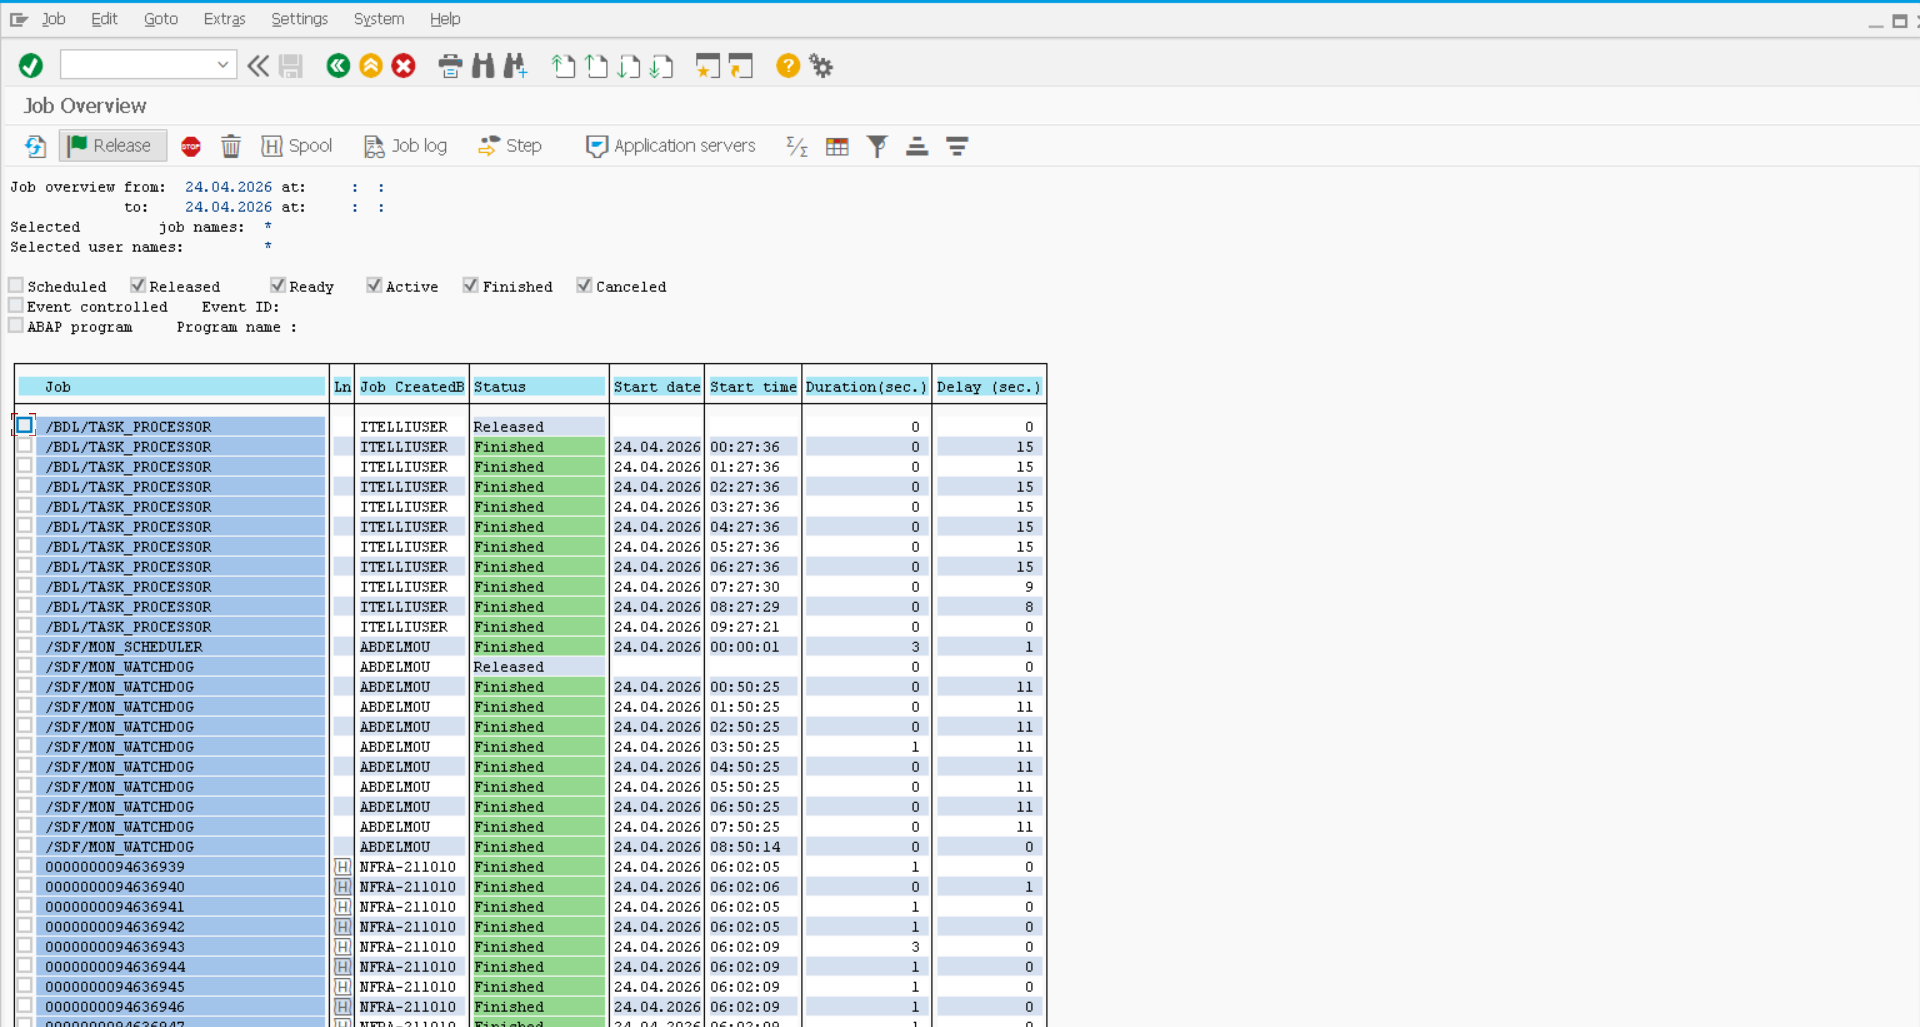
\includegraphics[width=\textwidth]{images/sm37.png}
  \caption{SM37 — Vue d'ensemble des jobs batch}
  \label{fig:sm37}
\end{figure}

La figure SM37 présente l'interface du T-code \texttt{SM37}, qui affiche
la liste des jobs planifiés avec leur statut (\textit{Finished}, \textit{Released},
\textit{Active}), leur date et heure de démarrage, leur durée d'exécution ainsi que
le délai éventuel. Cette vue permet à l'administrateur BASIS d'identifier en un coup
d'œil tout job bloqué, annulé ou présentant un délai anormal, et d'intervenir
rapidement avant que cela n'impacte les processus métier.

% ---- DB02 ----
\subsubsection*{DB02 — Space Overview}

DB02 surveille la base de données — l'administrateur contrôle l'espace disque
disponible pour éviter que la base de données sature, ce qui provoquerait un
arrêt complet du système.

\begin{figure}[H]
  \centering
  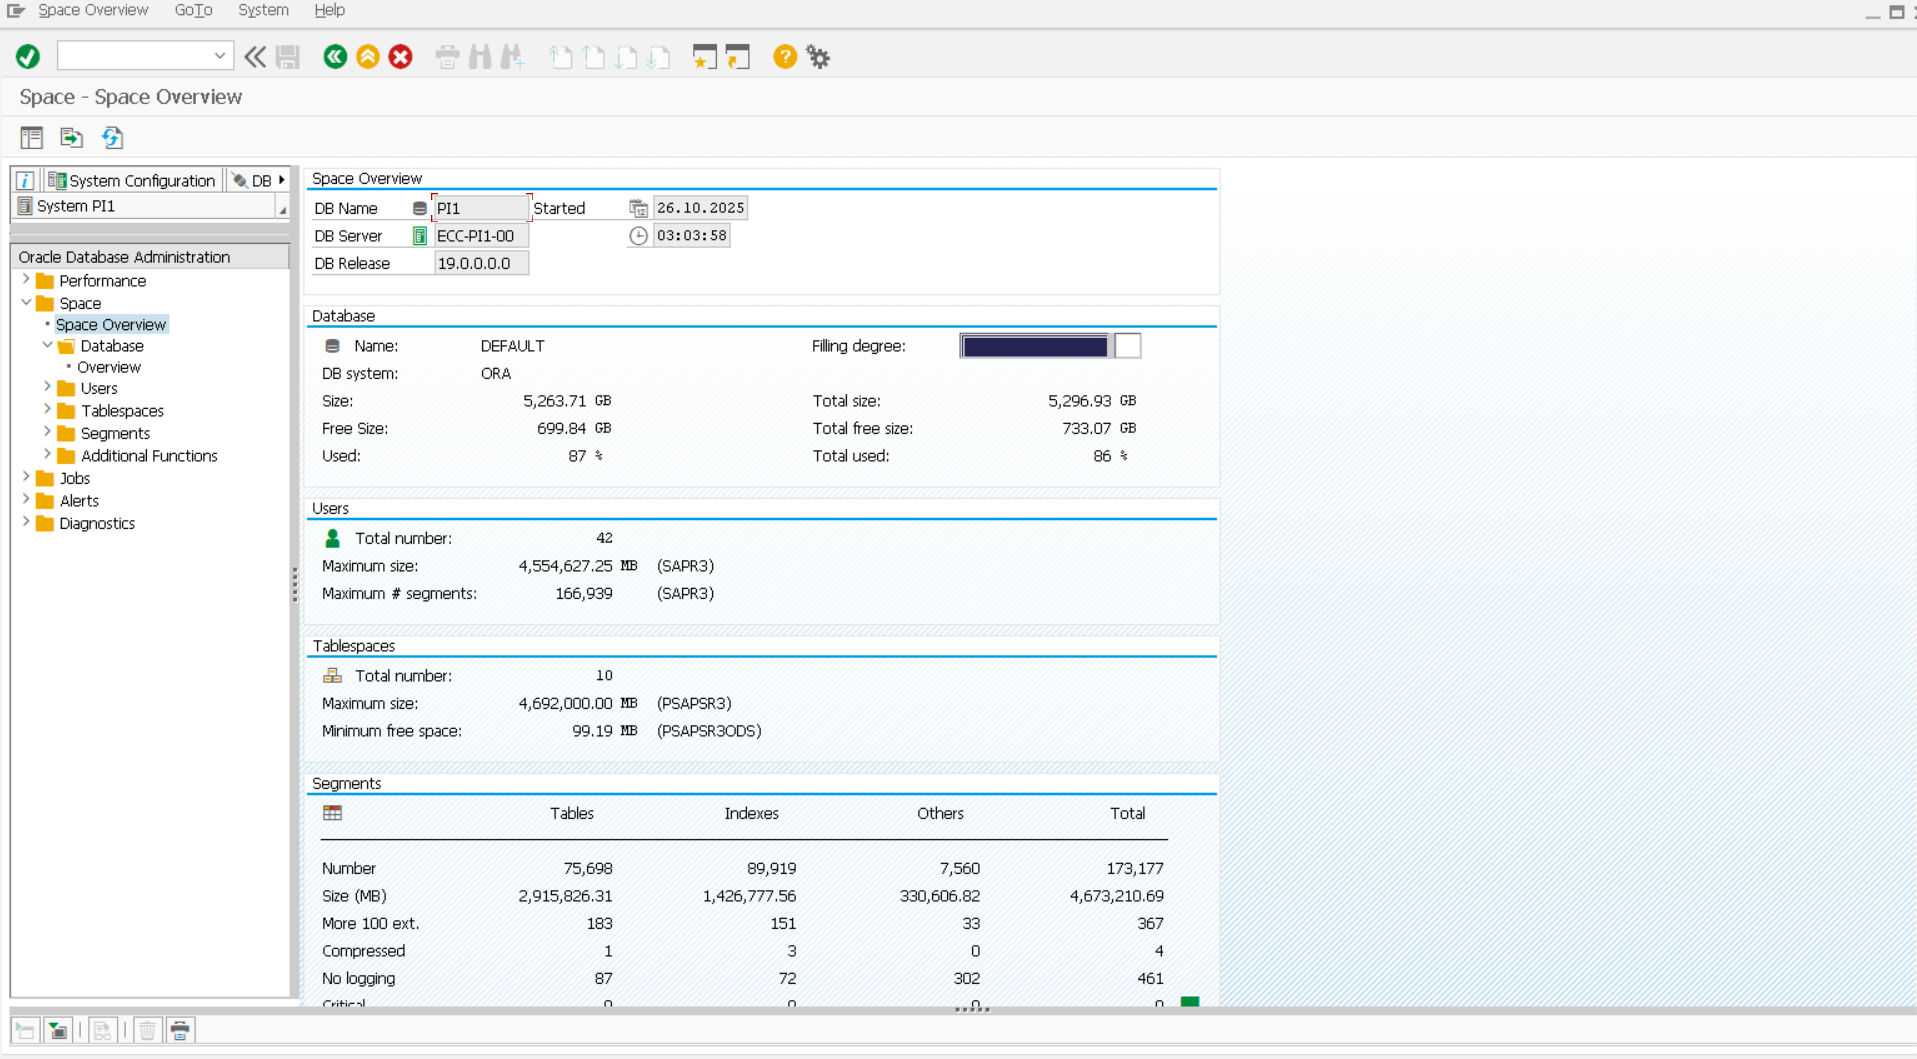
\includegraphics[width=\textwidth]{images/db02.png}
  \caption{DB02 — Vue d'ensemble de l'espace base de données}
  \label{fig:db02}
\end{figure}

La figure db02 illustre le T-code \texttt{DB02}, qui fournit une vue
synthétique de l'état de la base de données Oracle. On y retrouve le taux de
remplissage global, la taille totale et l'espace libre, ainsi que le détail par
tablespace et par segment (tables, index, autres). Un taux d'utilisation élevé —
comme les 87\% visibles ici — constitue un signal d'alerte critique nécessitant
une action immédiate d'extension ou de purge pour prévenir toute saturation du système.

% ---- ST22 ----
\subsubsection*{ST22 — Runtime Errors}

ST22 liste les erreurs critiques ABAP — l'administrateur analyse les
\textit{dumps} pour identifier les programmes qui plantent et corriger
les problèmes avant qu'ils n'impactent les utilisateurs.

\begin{figure}[H]
  \centering
  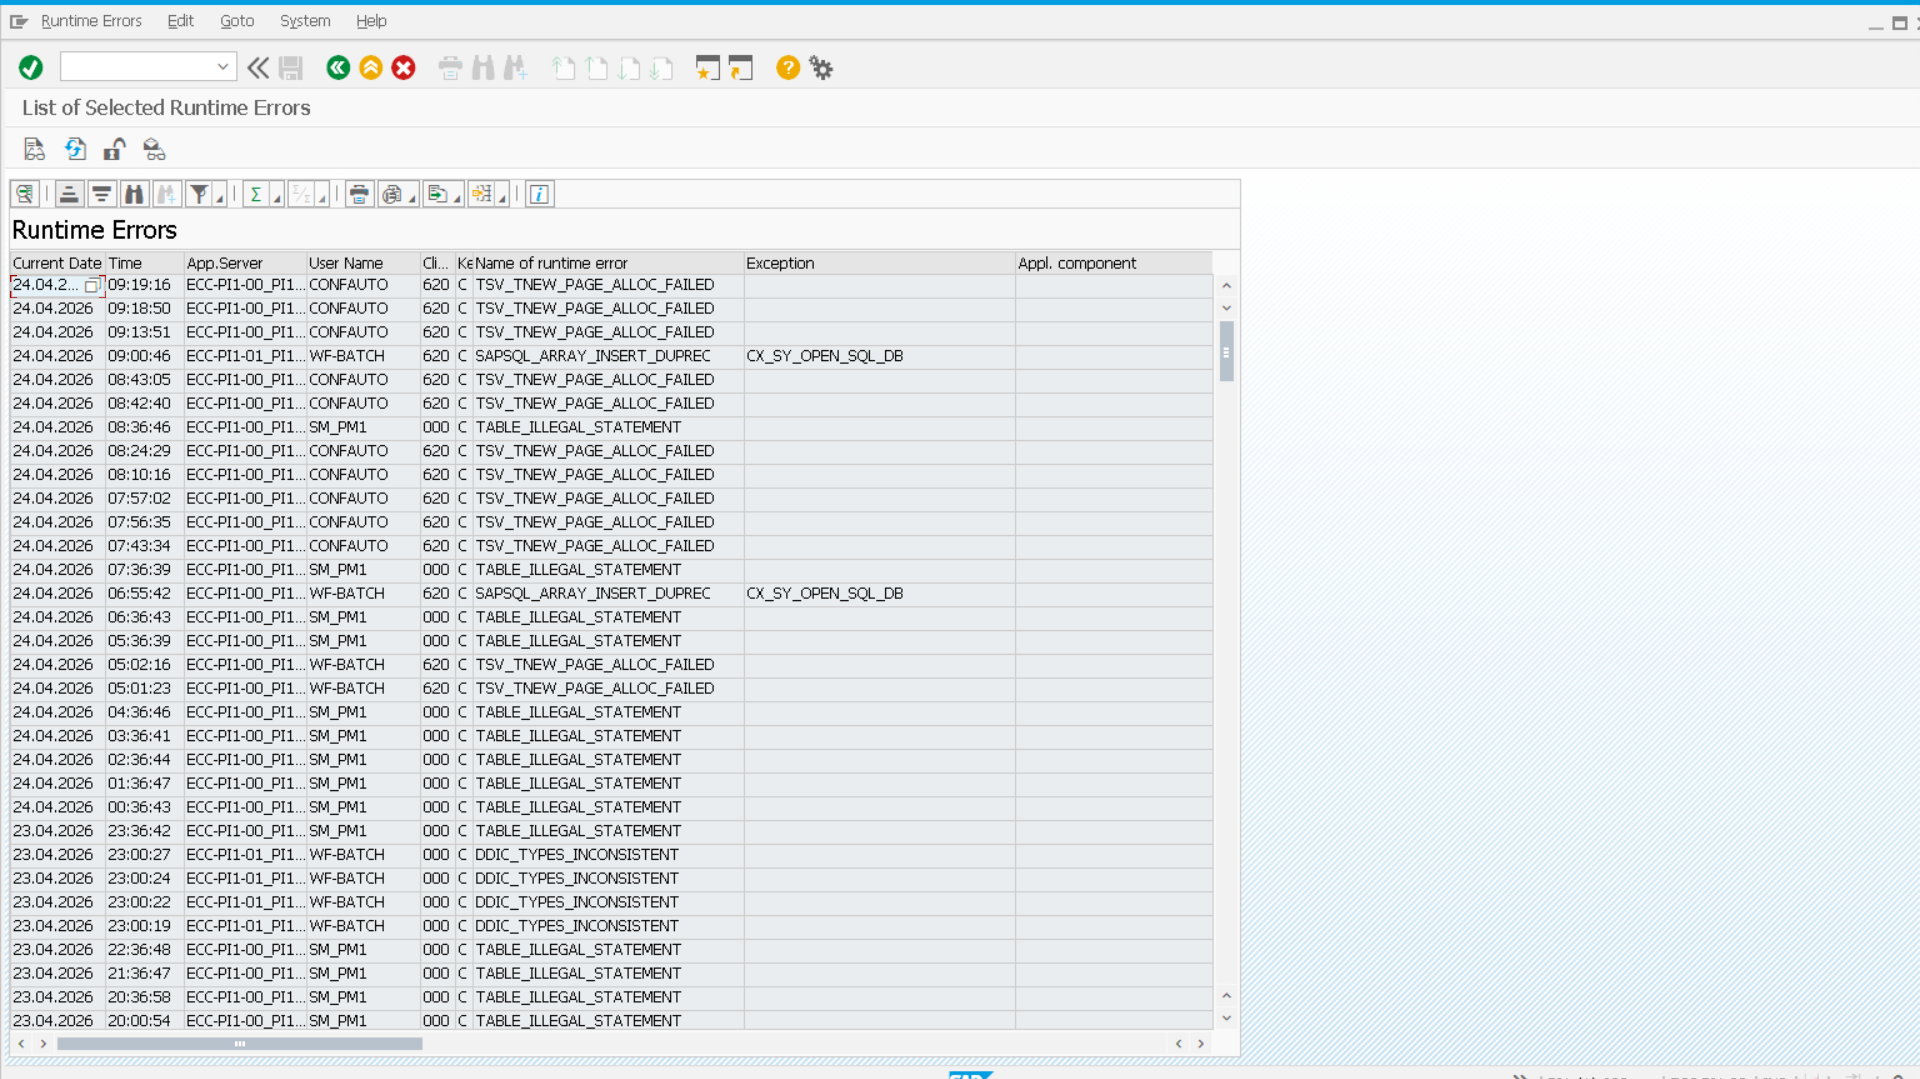
\includegraphics[width=\textwidth]{images/st22.png}
  \caption{ST22 — Liste des erreurs d'exécution ABAP}
  \label{fig:st22}
\end{figure}

La figure ST22 présente l'interface du T-code \texttt{ST22}, qui recense
l'ensemble des \textit{short dumps} ABAP survenus sur le système. Chaque entrée
indique la date, l'heure, le serveur applicatif, l'utilisateur concerné et le nom
de l'erreur. Les erreurs récurrentes telles que \texttt{TSV\_TNEW\_PAGE\_ALLOC\_FAILED}
(manque de mémoire) ou \texttt{TABLE\_ILLEGAL\_STATEMENT} (instruction SQL non autorisée)
sont des indicateurs d'anomalies systémiques qui doivent être analysées et résolues
en priorité par l'équipe BASIS.

% ============================================================
\subsection{Les Fondements Technologiques de l'IA Générative}

L'intelligence artificielle générative s'appuie sur une série de composants technologiques
complémentaires qui, lorsqu'ils sont assemblés, permettent la création de systèmes capables
d'interpréter, de raisonner et de produire du contenu à partir de données complexes. Ce
rapport se concentre sur deux éléments essentiels : les modèles de langage de grande taille
(LLMs), qui assurent la compréhension et la génération, et l'architecture RAG
(\textit{Retrieval-Augmented Generation}), qui améliore ces modèles en leur offrant une
base de savoir actualisée et vérifiable.

% ============================================================
\subsection{Architecture de l'IA RAG}

Un grand modèle de langage (LLM) détient une compréhension générale acquise lors de son
entraînement, mais il n'a pas d'accès direct à vos documents internes, à vos bases de
données confidentielles ou aux informations les plus récentes. L'architecture RAG
(\textit{Retrieval-Augmented Generation}) pallie cette lacune : avant de générer une
réponse, le système découpe d'abord les documents sources en fragments appelés
\textit{chunks} — de courts passages de quelques phrases ou paragraphes —, puis transforme
chacun d'eux en un \textit{embedding}, c'est-à-dire un vecteur numérique qui encode le
sens du texte plutôt que ses mots exacts. Ces vecteurs sont stockés dans une base de
données vectorielle, qui permet de retrouver en quelques millisecondes les chunks
sémantiquement les plus proches d'une question donnée, grâce à une mesure de similarité
cosinus. On peut percevoir le RAG comme un assistant disposant de sa propre bibliothèque :
au lieu de répondre directement de mémoire, il consulte d'abord les bonnes références,
extrait les passages essentiels, les injecte dans son contexte, puis construit une réponse
ancrée sur des faits vérifiables et traçables.
\begin{figure}[H]
  \centering
  \resizebox{\textwidth}{!}{%
  \begin{tikzpicture}[
      node distance=0.8cm and 1.5cm,
      box/.style={
          draw,
          rounded corners=8pt,
          minimum width=3cm,
          minimum height=1cm,
          align=center,
          font=\normalsize\bfseries,
          line width=1.2pt
      },
      arrow/.style={-Latex, line width=1.5pt},
      label/.style={font=\small, midway}
  ]

  % ══════════════════════════════
  % LIGNE 1 (haut) : Indexation
  % ══════════════════════════════
  \node[box, fill=yellow!40, draw=yellow!80!black] (docs)
      {Documents};

  \node[box, fill=blue!25, draw=blue!70, right=2cm of docs] (chunking)
      {Chunking};

  \node[box, fill=purple!25, draw=purple!70, right=2cm of chunking] (embedding)
      {Embeddings};

  \node[box, fill=green!30, draw=green!70, right=2cm of embedding] (vector)
      {Vector DB};

  % ══════════════════════════════
  % LIGNE 2 (bas) : Génération
  % ══════════════════════════════
  \node[box, fill=red!20, draw=red!70, below=2.5cm of vector] (retrieval)
      {Top-K \\ Retrieval};

  \node[box, fill=orange!30, draw=orange!80, left=2cm of retrieval] (llm)
      {LLM};

  \node[box, fill=cyan!25, draw=cyan!70, left=2cm of llm] (response)
      {Response};

  % ══════════════════════════════
  % USER QUERY : centré verticalement
  % ══════════════════════════════
  \node[box, fill=gray!20, draw=gray!60,
        below=2.5cm of embedding] (query)
      {User Query};

  % ══════════════════════════════
  % FLÈCHES — Indexation (ligne 1)
  % ══════════════════════════════
  \draw[arrow, blue!80]
      (docs) -- node[label, above]{\small découpage} (chunking);

  \draw[arrow, purple!80]
      (chunking) -- node[label, above]{\small vectorisation} (embedding);

  \draw[arrow, green!80]
      (embedding) -- node[label, above]{\small stockage} (vector);

  % ══════════════════════════════
  % FLÈCHES — Génération (ligne 2)
  % ══════════════════════════════
  \draw[arrow, red!80]
      (vector) -- node[label, right]{\small similarité} (retrieval);

  \draw[arrow, orange!80]
      (retrieval) -- node[label, below]{\small contexte} (llm);

  \draw[arrow, cyan!80]
      (llm) -- node[label, below]{\small génération} (response);

  % ══════════════════════════════
  % FLÈCHES — User Query
  % ══════════════════════════════
  \draw[arrow, dashed, gray!70]
      (query) -- node[label, right]{\small recherche} (vector);

  \draw[arrow, gray!70]
      (query) -- node[label, right]{\small prompt} (llm);

  \end{tikzpicture}%
  }

  \caption{Pipeline RAG : indexation, vectorisation, récupération et génération}
  \label{fig:rag_pipeline}
\end{figure}

% ============================================================
\subsection{Large Language Models (LLMs)}

Un LLM (\textit{Large Language Model}) est un type de modèle d'intelligence artificielle
qui a été formé sur d'énormes volumes de textes — tels que livres, articles, sites
internet, code — dans le but de comprendre les structures, les significations et les
connexions entre les mots d'une langue. En pratique, il anticipe le terme (ou jeton) le
plus susceptible de suivre un certain texte et c'est en répétant ce processus des milliers
de fois qu'il produit des réponses cohérentes, rédige des documents, fait des traductions,
résume ou répond à des interrogations. Plus le modèle est vaste (comportant des milliards
de paramètres), plus il a la capacité de saisir les subtilités complexes du langage. Des
exemples de LLM accessibles au public comprennent ChatGPT, Claude et Gemini.

% ============================================================
\section*{Conclusion}
\addcontentsline{toc}{section}{Conclusion}

Ce chapitre souligne l'importance stratégique du développement d'un système de détection
d'anomalies adapté aux transactions SAP dans le cadre de la méthodologie CRISP-DM. En
alignant les capacités techniques sur les objectifs métier, ce projet vise à améliorer
l'efficacité opérationnelle des équipes BASIS, à optimiser les processus de prise de
décision et à réduire le temps moyen de résolution des incidents.